%diploma-vaz fo dokumentum
%Keszult: 2004. februar
%(c) Markus Janos, http://mit.bme.hu/~markus, markus@mit.bme.hu
%Tesztelve: Miktex 2.3 alatt

%\documentclass[12pt,a4paper,twoside,openright]{report}  %Ketoldalas szedes
\documentclass[12pt,a4paper,oneside]{report}            %Egyoldalas szedes

%%Itt kivalaszthatjuk az egyes fejezeteket, ha nem akarjuk az egeszet forditani
%\includeonly{01_elozm, 02_eloszo, 03_1fej}

\usepackage{bmedipl}         %margo-, nyelv es egyeb allitas

%\usepackage{amsmath}         %matematikai segelycsomag
\usepackage{graphicx}        %grafikai
\usepackage{amssymb}
\usepackage{listings}
\usepackage{booktabs}
\usepackage{ltablex}
\usepackage{tikz}
\lstset{numbers=left, numberstyle=\tiny, basicstyle=\ttfamily, breaklines=true, frame=single, tabsize=2}

\usepackage{setspace}         %1.5-os, 2-es sorkoz hasznalatahoz.
                              %Ettol a tablazatok, abrak, labjegyzetek maradnak 1-es sorkozzel!
\onehalfspacing               %1.5-os sortav. Nem kotelezo szerintem...
%\doublespacing                %2-es sortav. Csak korrekturahoz!...

%\usepackage[dcu]{harvard}    %harvard tipusu hivatkozashoz (ld. a dokumentaciojat)
% \citationstyle{dcu}
% \citationmode{abbr}
% \harvardparenthesis{square}
% \harvardyearparenthesis{round}
% \renewcommand{\harvardand}{\'es}


%a jelolt neve
\renewcommand{\nev}{András Veres-Szentkirályi}

%konzulens adatai
\renewcommand{\konzulens}{Balázs Simon}
\renewcommand{\konzbeoszt}{PhD student}

%a dolgozat cime, ev
\renewcommand{\cim}{Extending Python Web Services}
\renewcommand{\ev}{2011.}

\hyphenation{meg-szentség-te-le-nít-he-tet-len}  %egyedi elvalasztas

\usepackage[
  unicode=true,
  colorlinks=false,
  pdfborder={0 0 0 0},
  pdfauthor={\nev},
  pdftitle={\cim}
]{hyperref}
\usepackage[all]{hypcap}

\begin{document}

\pagenumbering{roman}
%%%%%%%%%%%%%%%%%%%%%%%%%%%
% Diplomaterv-kiiras (ezt adjak, bele kell kötni a diplomába)
%%%%%%%%%%%%%%%%%%%%%%%%%%%
\begin{center}

\textbf{BUDAPEST UNIVERSITY OF TECHNOLOGY AND ECONOMICS}

\medskip


\includegraphics[width=8.79cm]{images/bme.pdf}

\medskip

\textbf{FACULTY OF ELECTRICAL ENGINEERING AND INFORMATICS\\SOFTWARE ENGINEERING}

 \vspace{2cm}
 \Large\textbf{\cim}

 \vspace{6mm}
 \textbf{\nev} \\
 \texttt{<vsza@vsza.hu>} \\ \strut \\

 \Large\textbf{MSc. Thesis}

\end{center}

\vfill

Consultant:

\begin{center}
\konzulens\\ \konzbeoszt

\vspace{96pt}

December 2011
\end{center}

% \vspace{6mm}
% \begin{tabular}{p{80mm}l}
% A záróvizsga tárgyai:   & Első tárgy \\
%                         & Második tárgy \\
%                         & Harmadik tárgy
%  \end{tabular}
%
%  \vspace{6mm}
%  \begin{tabular}{p{80mm}l}
%  A tervfeladat kiadásának napja:         &  \\
%  A tervfeladat beadásának határideje:    &
%  \end{tabular}
%
% \vfill
%
% \begin{center}
% \begin{tabular}{cc}
%  \makebox[7cm]{\emph{dr.\ Görgényi András}}    & \makebox[7cm]{\emph{dr.\ Péceli Gábor}} \\
%  \makebox[7cm]{adjunktus, diplomaterv felelős} & \makebox[7cm]{egyetemi tanár, tanszékvezető}
% \end{tabular}
% \end{center}
%
%  \vspace{6mm}
%  \begin{tabular}{p{80mm}l}
%  A tervet bevette:           & \\
%  A terv beadásának dátuma:   & \\
%  A terv bírálója:            &
%  \end{tabular}


 \thispagestyle{empty}
 \blankpage

\selectlanguage{magyar}
%%%%%%%%%%%%%%%%%%%%%%%%%%%
% Diplomaterv-kiiras melleklete (ezt is adjak, bele kell kötni a diplomába)
%%%%%%%%%%%%%%%%%%%%%%%%%%%
 \begin{textblock*}{\paperwidth}(0mm,0mm)
    \noindent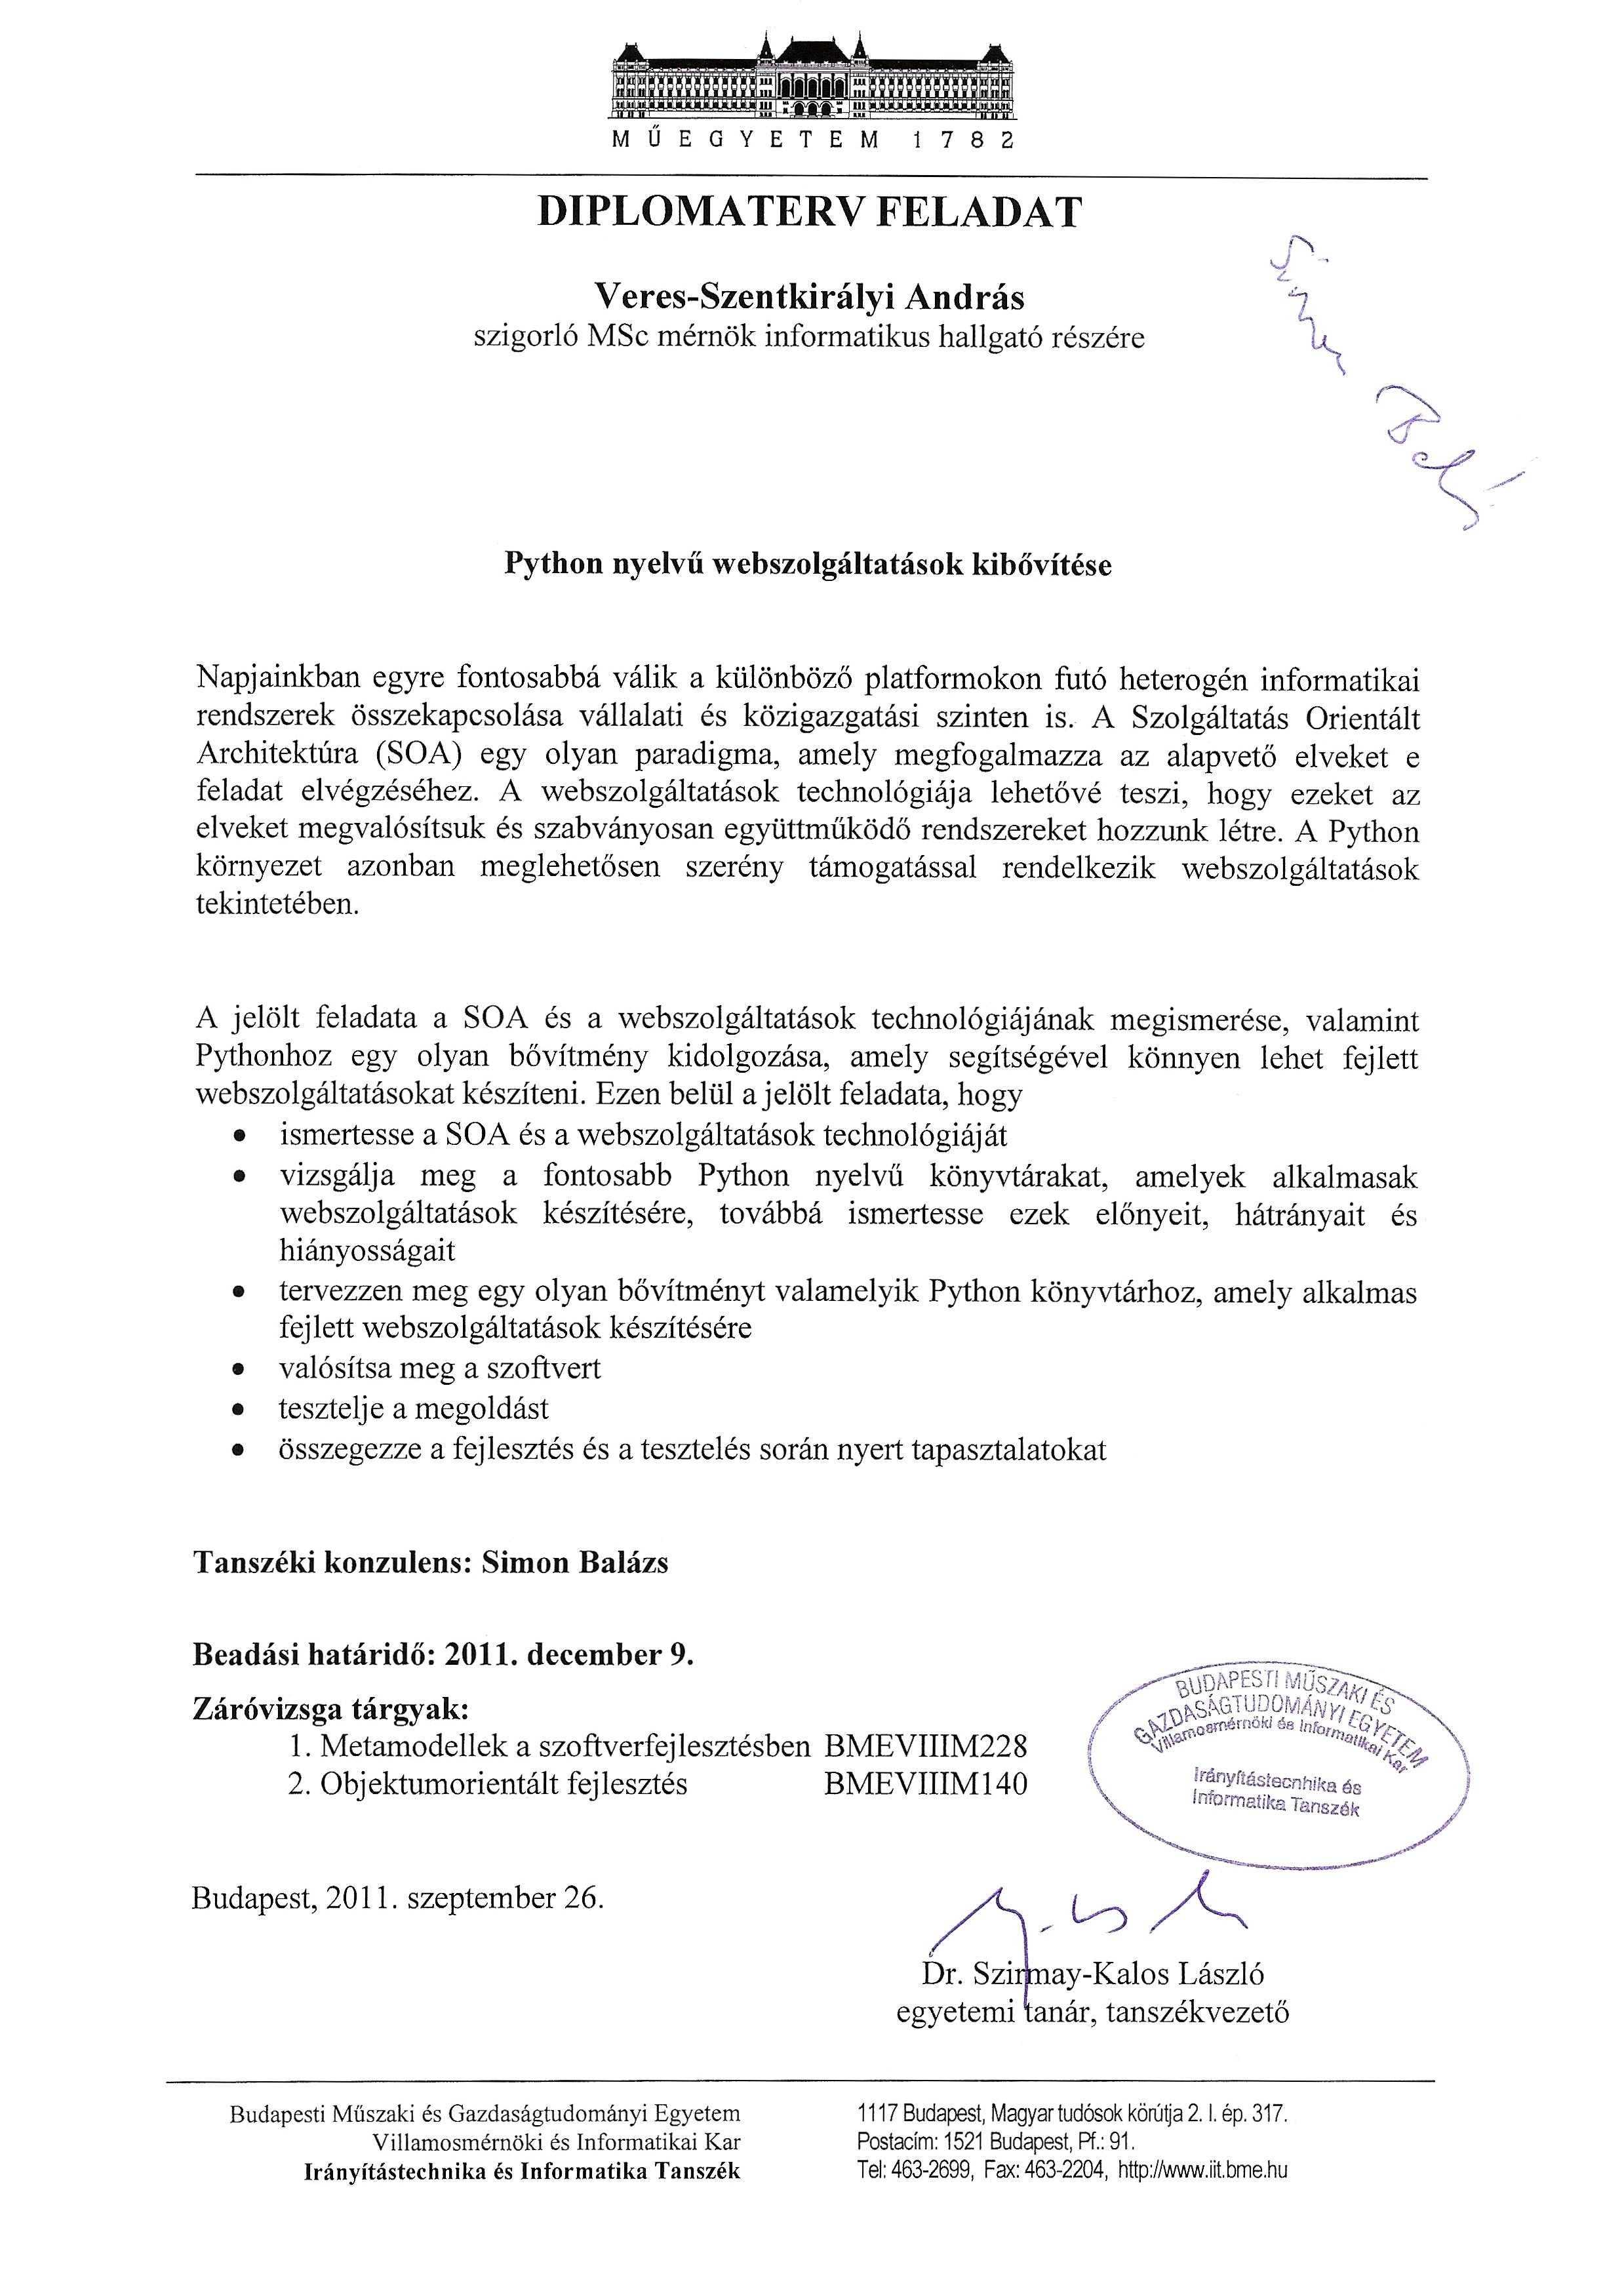
\includegraphics[width=\paperwidth,height=\paperheight]{images/feladat-retouched.jpg}
	\end{textblock*}
	\mbox{}
 \blankpage

%%%%%%%%%%%%%%%%%%%%%%%%%%%
% Nyilatkozat
%%%%%%%%%%%%%%%%%%%%%%%%%%%
\def\abstractname{Nyilatkozat}
\begin{abstract}

\noindent
Alulírott \emph{Veres-Szentkirályi András}, szigorló hallgató kijelentem,
hogy ezt a diplomatervet meg nem engedett segítség nélkül, saját  magam
készítettem, csak a megadott forrásokat (szakirodalom, eszközök, stb.)
használtam fel. Minden olyan  részt, amelyet szó szerint, vagy azonos
értelemben, de átfogalmazva más forrásból átvettem, egyértelműen, a
forrás megadásával megjelöltem.

\begin{flushright}
 \vspace*{1cm}
 \makebox[7cm]{\rule{6cm}{.4pt}}\\
 \makebox[7cm]{\emph{Veres-Szentkirályi András}}\\
 \makebox[7cm]{hallgató}
\end{flushright}
\end{abstract}

%%%%%%%%%%%%%%%%%%%%%%%%%%%
% Tartalomjegyzek
%%%%%%%%%%%%%%%%%%%%%%%%%%%
\selectlanguage{english}
\tableofcontents

%%%%%%%%%%%%%%%%%%%%%%%%%%%
% Kivonat
%%%%%%%%%%%%%%%%%%%%%%%%%%%
\def\abstractname{Kivonat}
\selectlanguage{magyar}
\begin{abstract}
\addcontentsline{toc}{chapter}{Kivonat}
% TODO
\end{abstract}


%%%%%%%%%%%%%%%%%%%%%%%%%%%
% Abstract
%%%%%%%%%%%%%%%%%%%%%%%%%%%
\selectlanguage{english}
\begin{abstract}
\addcontentsline{toc}{chapter}{Abstract}
% TODO
\end{abstract}
      %elso lapok (Cimlap, kiiras, tartalomjegyzek, Kivonat, Abstract,egyeb)
%%Eloszo

\chapter*{Introduction}

 \addcontentsline{toc}{chapter}{Introduction}
 \markboth{\uppercase{Introduction}}{\uppercase{Introduction}}
 \pagenumbering{arabic}

% background in five paragraphs
Looking at the history of ITC systems, interoperability was not a big issue at the beginning -- simple systems can communicate using primitive methods. As time went by, systems evolved, and innovation lead to such diversity, that made high level interconnection of systems a major headache of system integrators. Naturally, the market reacted and came up with various solutions, well distributed along the scale of bloatedness, including DCOM, CORBA and XML-RPC.

These competing solutions were and are more or less usable within their scopes, limited by platform-dependence, but more importantly the inability to operate over the Internet -- either because of the incompatibility with appliances at network borders, or because of security issues. The World Wide Web brought simple open protocols, and mature solutions to pass its network traffic through network borders, making it an ideal choice as the transport layer for the next generation of interoperability platforms.

SOAP was created as the encoding method of request, reply and fault messages exchanged between services and consumers over the transport layer, but it didn't solve all problems in itself. For instance, trusting a network out of control of both parties required additional standardized ways of ensuring the confidentiality and integrity of the transmitted message, as well as authenticating the consumer and/or the service. In case of this problem, WS\hyp{}Security was born as a solution, providing a simple and open method of ensuring the necessary level of security for SOAP messages relayed over untrusted networks.

Python was one of the few languages, that -- despite its roots -- could emerge from the academic circles, and found its way to developers, hackers, and system administrators alike. The rich set of libraries and sane design made it a perfect choice for high-level implementation, allowing a smooth transition from ideas through prototypes to solutions ready for deployment -- the same feature that caused many people writing it off as a ``scripting language''. As was Java before the millennium, Python is currently considered by many as the language of the Internet (or at least one of them), which means, advanced SOAP support is a must-have in order for Python to be accepted as the foundation of a wider range of systems.

One of the negative side effects of the community-driven development of the Python ecosystem is that features needed by less people get a smaller fraction of developer attention -- and this was exactly the fate of advanced Python SOA implementations. Although SOAP libraries did exist, their support was limited to the level the developer(s) required, resulting in many organizations choosing other platforms solely based on their advanced SOAP support -- creating a situation I refused to accept.

% sum of chapters in two paragraphs
The first chapter introduces the Service-oriented Architecture and web services, including their brief history and principles. Using these as a basis, the scope is first focused on advanced web services, and then on the security of web services. The second chapter sheds some light on the other half of the thesis title, Python, and presents the available SOA solutions compatible with the platform, along with their advantages and disadvantages. The chapter ends with a quick summary of the Python SOA landscape, picking SUDS as a suitable base of improvement.

The third chapter goes into detail about SUDS, starting with its interface presented to the developer, then focusing on the security-related parts of its internals, ending in its interesting stubs awaiting improvement. The fourth chapter starts from the deficiencies of SUDS, and introduces the component I designed to enable advanced web service consumptions. In the second half of the chapter, a testbed is shown, which I developed to make sure, that the result of the improvement is able to interoperate with services correctly. The fifth chapter demonstrates the measurements I did to evaluate the quality of my solution, and the sixth closes the thesis study by summarizing the development process and its results, offering future improvement ideas to address the remaining issues.
     %Eloszo, ebben celkituzes, elozmenyek, felepites, koszonetnyilvanitas
                        %max. nehany oldal

%\chapter{Service-oriented Architecture and Web Services}

\section{SOA history and principles}

As \cite{soa_modeling} remembers, not long after the new millenium, the world of IT got fed up with interoperability, reusability, and other issues -- and Service-oriented Architecture was born. The paradigm was was built upon the foundations of IT best practices of its time, and tried to encourage software design made of loosely coupled components. Reduction of time to market and business agility are advantages, that are obvious to both business and IT people. This step is a logical one in the course of software engineering history -- states \cite{devcom_soa_intro}. The technological shifts always followed the increasing software complexity, from functions, through classes, to components. But even the users of components are tied to the technology (runtime, platform) the component uses. According to \cite{ibm_soa_impro}, SOA addresses this problem by the following guiding principles.

\begin{itemize}
 \item Reuse, granularity, modularity, composability, and componentization
 \item Compliance to standards (both common and industry-specific)
 \item Services identification and categorization, provisioning and delivery, and monitoring and tracking
\end{itemize}

\section{Web Services}

Many technologies tried to implement SOA (or something close), for example Microsoft's DCOM and OMG's CORBA also offered a somewhat standardized way for entities (components, services) to interoperate. One of the problems were the limitations of the implementations -- DCOM obviously depended on Windows as a platform, and although CORBA had (and has) ORB implementations available to several platforms and under diverse licensing, but the interoperability between these was often an issue. An even more troubling problem was the communications foundation of these solutions. Most of these (DCOM and CORBA at least for sure) used a binary protocol and required direct connections to TCP ports -- sufficient for components communicating within the local corporate network, but unimaginable over the internet.

The World Wide Web introduced HTTP as a transport protocol, one especially designed for use over the internet. Besides that, corporate networks could also make use of it, since proxy servers could be installed, with the option of inspection, forwarding, filtering, and mangling of content passing through. These two properties made it a great foundation for interoperation, since the protocol allows any kind of content to be transferred, regardless of its type.

In a wide sense, every service, that is available for invocation through HTTP can be considered a web service, regardless of the layer used above HTTP. XML-RPC was the first such ``payload'', and as the name suggests, its semantics were based on method invocation. The structure is suprisingly simple, the method name and parameters are transmitted as the body of an HTTP request, and the body of the response contains the return value(s), both serialized using XML. A sample transcript can be seen on Figure \ref{fig:xmlrpc-sample}.

\begin{figure}[htbp]
 \centering
 \begin{minipage}[t]{0.56\linewidth}
  \centering
  \begin{lstlisting}[language=XML, numbers=off]
<?xml version="1.0"?>
<methodCall>
 <methodName>getPop</methodName>
 <params>
  <param>
   <value>
    <string>Budapest</string>
   </value>
  </param>
 </params>
</methodCall>
  \end{lstlisting}
 \end{minipage}
 \hspace{0.5cm}
 \begin{minipage}[t]{0.37\linewidth}
  \centering
  \begin{lstlisting}[language=XML, numbers=off]
<?xml version="1.0"?>
<methodResponse>
 <params>
  <param>
   <value>
    <i4>1733685</i4>
   </value>
  </param>
 </params>
</methodResponse>
  \end{lstlisting}
 \end{minipage}
 \caption{Transcript of an XML-RPC method invocation}
 \label{fig:xmlrpc-sample}
\end{figure}

\section{SOAP and friends}

\begin{figure}[htbp]
 \centering
 \begin{minipage}[t]{0.47\linewidth}
  \centering
  \begin{lstlisting}[language=XML, numbers=off]
<soap:Envelope xmlns:soap="http://schemas.xmlsoap.org/soap/envelope/">
 <soap:Body>
  <bme:getPop xmlns:bme="http://vsza.hu/bme">
   <city>Budapest</city>
  </bme:getPop>
 </soap:Body>
</soap:Envelope>
  \end{lstlisting}
 \end{minipage}
 \hspace{0.5cm}
 \begin{minipage}[t]{0.47\linewidth}
  \centering
  \begin{lstlisting}[language=XML, numbers=off]
<soap:Envelope xmlns:soap="http://schemas.xmlsoap.org/soap/envelope/">
 <soap:Body>
  <bme:getPopResponse xmlns:bme="http://vsza.hu/bme">
   <return>1733685</return>
  </bme:getPopResponse>
 </soap:Body>
</soap:Envelope>
  \end{lstlisting}
 \end{minipage}
 \caption{Transcript of a SOAP method invocation}
 \label{fig:soap-sample}
\end{figure}

As \cite{box_soap_history} wrote, SOAP has evolved from XML-RPC inside Microsoft -- the base operation remained the same, the method identification and parameters are serialized using XML, and so is the response. One notable difference is the absence of XML header (SOAP uses UTF-8 encoding implicitly) and the extensive use of XML namespaces, as it can be seen on Figure \ref{fig:soap-sample}. W3C took control of the specification, and SOAP became the encoding of web services, with usually HTTP(S) or SMTP as the underlying transport mechanism. WSDL was born to describe the interface of web services, using XML again. Although other technologies appeared (such as UDDI for service discovery) the two dominant players in web services are SOAP and WSDL.

WSDL is usually automatically generated from services written in any programming language. Client libraries running on platforms supporting dynamic dispatch (such as Python, Ruby, PHP) usually allow dynamic creation of service proxies for consumption using the WSDL. The other approach, available for all runtimes and most programming languages is automatized code generation, during which class hierarchies representing the service interfaces are generated for later used in compiled code. During invocation, the proxy serializes the platform-dependent data structures into a SOAP envelope, and transfers it to the service, which does the exact opposite by marshalling the parameters into native objects. This way, both the service and the consumer code handles entities that are native to the platform they're dependent on, and can interoperate with each other, without any prior knowledge of the technology powering the ``other side''.

\section{Advanced web services}

\subsection{Introduction}

Using WSDL as a machine-parseable, standardized form of service descriptor was a vast improvement on the way of web services from XML-RPC to SOAP. W3C and OASIS standardized many additional methods of improving web services, such as metadata exchange, security, and reliable messaging. On the bright side, these make it possible to build advanced services while maintaining responsibility separation (implementation focuses on business logic) and without sacrificing interoperability. But on the other hand, these standards are complex, and continuously evolve -- a great example is WS-Reliability vs. WS-ReliableMessaging -- so not every SOAP implementation support everything, which in turn limits interoperability and thus platform independence.

\subsection{Security}

During the course of my thesis, I focused on the technologies for securing web services. When introducing this area to people, many reply with ``just use HTTPS'', which indeed provides transport security between two hosts. The problem with that approach is that one of the key features of web services is the ability to interconnect services and consumers in different networks, which means, that the network traffic might have to pass through HTTP proxies and other advanced network appliances. This makes HTTPS inadequate to establish a secure (authenticated, digitally signed, and/or encrypted) end-to-end connection, so the problem has to be solved inside SOAP, and HTTPS can only be thought as an outer layer of protection.

After initial development by IBM, Microsoft and Verisign, OASIS released WS\hyp{}Security 1.0 on April 19, 2004. It covers all three aspects I mentioned in the previous paragraph using the following technologies.

\begin{description}
 \item[Authentication] Security tokens can be attached to the SOAP message header for the sender to identify herself. This can be done using either username-password pairs (in plaintext or digested format) or by using a more heavyweight solution like X.509 or Kerberos.
 \item[Digital signature] Signatures can be attached to the SOAP message header in order to protect the integrity of the message and provide non-repudiation. It also supports many strategies, such as RSA, DSA or PGP keys.
 \item[Encryption] Any subset of the SOAP message can be encrypted, so that only the intended recipient has access to its contents. Since the current specification was found vulnerable to cryptanalisys by \cite{acm-xmlenc-breaking}, I ignored this part in my thesis.
\end{description}
       %elso fejezet: bevezetes
%\chapter{Existing Python SOA solutions}

\section{About Python}

\subsection{Language}

According to \cite{python-faq}, ``Python is an interpreted, interactive, object-oriented programming language''. What's missing from this self-description are those things, that make the language unique. The first thing most people recognize while reading a Python source code, is the use of indentation for structure markup. This feature might be odd and strict for first sight, but it makes code written by other people highly readable and reusable. The subsequent clean feeling of the code is strengthened even more by the availability of functional constructs, which give the right tools for most purposes into the hands of the developer. The essence of the language can be reduced to a single phrase, which can be interpreted in both positive and negative ways: ``executable pseudocode'' -- code snippets are explicit enough for most people (even those without Python knowledge) to understand.

\subsection{Runtime}

The first and most widely-used interpreter is called CPython, and it's the reference implementation of the language runtime. It compiles source code (\verb|.py| files) into bytecode (\verb|.pyc| files) for interpretation. It also provides an interactive shell, which can be used for experimentation or debug purposes. Because of this, the UNIX program loader can use it as a standard interpreter, so Python scripts prefixed with an appropriate shebang can be run directly. As the name suggests, the implementation is written in mostly C/C++, which causes built-in functions to perform well.

There are separate projects, that bridges the Python world with other solutions -- IronPython and Jython compiles Python code into .NET and Java bytecode, respectively, and Nokia ported Python to its S60 (Symbian) platform. This way, Python can interoperate with existing frameworks and libraries at a lower level, if needed. Another approach is outlined in the next subsection.

\subsection{Libraries}

Python comes with ``batteries included'' -- libraries are available for most purposes a developer might need, such as file manipulation, network connectivity, parsing and serializing from and to a variety of formats. Libraries can be either written in Python -- in which case, they are as portable as any other Python code between runtimes -- or using the C/C++ API. Thin, sometimes automatically generated libraries, that only wrap a certain native libraries are called bindings -- there's even a dialect of Python called Cython, that allows calling of C/C++ functions, and produces native code. Because of these features, although interpreted languages are usually suffer from poor performance, well-designed Python applications perform only high-level orchestration in the interpreted engine, and delegate computationally intensive tasks to native code. This design motivates developers to avoid premature optimization, while allowing fast prototyping and outstanding performance using the same foundations.

\section{Python SOA solutions}

\subsection{Introduction}

The community around the Python ecosystem is one of those closest to the ``free software culture'' envisioned by Richard M. Stallman and Eric S. Raymond. This results in libraries being written mostly out of curiosity and immediate need -- a good combination for a good base system, not so good for SOAP. Many other ways of remote method invocation are solved in Python libraries, but SOAP has maintained a low level of maturity. The basic invocation examples usually work, but the level of development clearly shows the needs of the developer.

This problem is partly caused by the network effect: if everybody uses .NET and Java for web service interoperation, if a platform needs to be chosen for a solution to access them, it usually seems logical for most people to choose one of the two heavyweight products. The other factor is the mindset of Python developers -- they usually like to build systems out of small, autonomous entities, interconnected by simple and trivial protocols, and SOAP is not the first thing that comes to mind with these features, despite the fact that it can be used wisely.

Of course, there are developers both working on and using SOA with Python, there's even a public mailing list dedicated for the purpose, archives and subscription are available at \url{http://mail.python.org/mailman/listinfo/soap}.

\subsection{SOAPy}

As \cite{so-206154} wrote, it was the best SOAP client in the Python ecosystem, but the project is abandoned. As no one maintains the codebase -- its homepage was last modified in 2001 -- it became incompatible with later Python releases, which makes it hard to use in modern environments. The Debian project doesn't even maintain a package, so the only way to install it is to download the tar.gz file (uploaded in April 27, 2001) and extract it manually.

I found its internal structure very simple -- the library consists of two Python source files, both under 500 lines of length. By looking at the import section, it was obvious, that it used libraries and functions, that are way obsolete now. Still, some of them are kept for the sake of backwards compatibility, but the PyXML package it used for XML processing is also no longer maintained, and had been removed from most major GNU/Linux distributions. The documentation -- including the examples -- suggested, that SOAPy offered client functionality only, and I didn't find any contradicting evidence in the source code.

\subsection{Zolera SOAP Infrastructure}
\label{ZSI}

ZSI is the other ``old boy'' among Python SOAP libraries. As \cite{pywebsvcs-talk} states, it way last fully released in 2007, but unlike SOAPy, it can be still used with recent Python environments. It offers two ways of operation: for simple services, it can construct the SOAP messages without a schema (Binding class), and for complex services, a proxy (ServiceProxy class) can be used to serialize arguments. It supports code generation from WSDL (\verb|wsdl2py|) and ``can also be used to build applications using SOAP Messages with Attachments'' \cite{zsi-doc}.

Ralf Schmitt wrote in \cite{zsi-velocity}, that ZSI is neither easy to set up and use, nor fast. I tried it anyway, and it was easy to install, since Debian still maintains a package. The first ServiceProxy example, which I took straight from the ZSI documentation failed, but I figured out, that they changed the structure, so I managed to run a test. It worked pretty well as a client, but it lacked any advanced debugging features -- for example, the list of methods could only be determined by listing the methods of the service proxy. Also, code (re)generation is necessary for complex data types, and is far from being trivial.

\subsection{soaplib / rpclib}

Soaplib focused on server-side SOAP implementation, using Python decorators, and provided WSGI-compatible services, so deployment was possible with both standalone processes or any WSGI-compatible web server (such as Apache \verb|mod_wsgi|). \cite{so-206154} wrote, that ``creating clients is a little bit more challenging'', so I looked through the documentation, and found, that according to \cite{soaplib2-changelog}, the developers did ``the right thing'' and shifted their entire focus on server implementation by dropping client functionality in favor of SUDS (see section \ref{suds}) at version 0.9.

The project was later renamed to rpclib, and widened its scope -- the old library only receives bug fixes, as the main developer focuses on the new one. I tried using it, and found it pleasant to use. Despite Python being a dynamically typed language, enabling code to be accessible via SOAP had not ``littered'' the code, and it offered automatic WSDL generation.

\subsection{SUDS}
\label{suds}

SUDS is a relatively new SOAP client library, compatible with Python 2.4 and newer releases. Its operation is like the proxy feature of ZSI, but it doesn't require any code generation. Complex classes can be assembled using the factory pattern, and while it might seem, that parsing WSDL and generating class hierarchy on-the-fly is slow, the built-in caching provides quite a performance. It supported several methods of authentication, including HTTP basic and digest, and also NTLM, which is necessary to consume Microsoft SharePoint web services. According to the general opinion of related forums and mailing lists (including \cite{so-206154}), SUDS is the preferred Python way of creating SOAP clients, and the library doesn't depend on obsolete components.

SUDS was released in a regular manner till 2010, and is available as a package in major Linux distributions. This way, installing the library was not a big issue, and the documentation \cite{suds-doc} covers all common use-cases. I tried it first with a basic invocation, and it worked as expected. Special methods were overridden in a way, that using the \verb|print| command on SUDS object rendered a nicely formatted, human readable printout, which makes debugging and experimentation much easier.

\subsection{sec-wall}

Although \cite{sec-wall-homepage} describing sec-wall as ``a security proxy that comes with tons of interesting features, very good documentation and an exceptionally friendly community'' might sound like the usual shameless self-promotion, this relatively new tool (1.0 released in April 2011) is a real gem. It acts as a proxy, thus enables the transformation of any SOAP backend into an advanced web service. Although written in Python could have meant poor performance, it takes the issue seriously and makes use of libraries that provide an native event-driven architecture.

I found it during the field-work, and I worked together with its author, Dariusz Suchojad to improve it -- one of the results were complete and correct UsernameToken support (both plain and digest), and an experimental digital signature implementation. Beside the performance and reusability, the quality of the software is also surprisingly great; it's built around the Python Spring Framework, making good use of the dependency injection feature, and its tests provide 100\% code coverage.

\subsection{Common problems}

While inspecting libraries offering both service and consumer functionality, unfortunately, they provided no or little support for advanced web services. SUDS offered UsernameToken, but didn't work in any mode, soaplib/rpclib and ZSI didn't even mention the possibility of such solutions -- although ZSI had some unused code implementing XML canonicalization. SOAPy barely even implemented SOAP -- besides it's unusable in modern environments. Although sec-wall solves the situation by providing proxy support, the problem of the client side remains -- and that's exactly, why I decided, to take a close look into SUDS.
       %masodik fejezet: a problema reszletes kifejtese
%\chapter{Opportunities and internals of SUDS}

\section{Introduction}

As I described in section \ref{suds}, SUDS is the de facto way of consuming web services in Python. One of the most compelling features lies within its simplicity and user friendliness. These help in the beginning, by making it really easy to create a working prototype in no time, both by using the interactive shell and writing scripts -- but later, the code is still readable, and at the same time, caching helps eliminating the performance trade-off. A sample run, consuming a currency rate service using SUDS in the interactive Python shell can be seen in Figure \ref{fig:suds-currency}.

\begin{figure}[htbp]
 \centering
\begin{lstlisting}[numbers=off, basicstyle=\footnotesize\ttfamily]
Python 2.7.2+ (default, Aug 16 2011, 07:03:08)
[GCC 4.6.1] on linux2
Type "help", "copyright", "credits" or "license" for more information.
>>> from suds.client import Client
>>> url = 'http://www.webservicex.net/CurrencyConvertor.asmx?WSDL'
>>> c = Client(url)
>>> print c

Suds ( https://fedorahosted.org/suds/ )  version: 0.4.1 (beta)  build: R703-20101015

Service ( CurrencyConvertor ) tns="http://www.webserviceX.NET/"
   Prefixes (1)
      ns0 = "http://www.webserviceX.NET/"
   Ports (2):
      (CurrencyConvertorSoap)
         Methods (1):
            ConversionRate(Currency FromCurrency, Currency ToCurrency, )
         Types (1):
            Currency
      (CurrencyConvertorSoap12)
         Methods (1):
            ConversionRate(Currency FromCurrency, Currency ToCurrency, )
         Types (1):
            Currency


>>> c.service.ConversionRate('EUR', 'HUF')
315.6003
\end{lstlisting}
 \caption{Requesting currency conversion rate using SUDS}
 \label{fig:suds-currency}
\end{figure}

\section{Internal structure}

In order to improve SUDS, I had to discover its inner workings -- the documentation covered standard use-cases pretty well, but told little about architecture. I split the code in time domain into two pieces, the separator being the end of \emph{suds.client.Client} object instatiation. Before that, WSDL fetching and parsing happens, and afterwards, during invocations, SOAP messages are built, sent, and responses are parsed and returned.

\subsection{Client proxy instantiation}

The \emph{Client} object is the ``soul'' of the library and can be found in the \emph{suds.client} module. The constructor has one fixed parameter (the WSDL URL), all the others get stored in a dictionary for later use. Upon creation, the WSDL gets fetched and all the plugins (see section \ref{sudsPlugins}) are notified. The WSDL is parsed for service definitions and schemas -- these are used to create the factories later used for the instatiation of complex objects, and for lookup on method invocation. The root element of the DOM representing the WSDL is stored for the whole lifecycle of the object in the \emph{wsdl} attribute, and the \emph{services} attribute is set to an instance of \emph{ServiceSelector}, the key to method invocation (see section \ref{sudsInvocation}).

\subsection{Instantiation of complex objects}

Since many web services expect complex objects as an input parameter, its instantiation is a problem present in all web services clients. As I mentioned in section \ref{ZSI}, ZSI solved this problem in the ``classic'' way, with source code generation, which makes experimentation teadious and increases turnaround times. In contrast, SUDS offers a solution implementing the Factory pattern, a ``method'' (actually a callable attribute) of the \emph{Client} class, which returns an appropriate object, given a class name. This object can be later populated as a regular object, or its attributes can be used in case of enumerations. Since version 0.3.8, SUDS also supports the automatic conversion of native Python dictionary objects to SOAP complex types, using the keys as attribute names, which can lead to cleaner code in some cases.

\subsection{Service method invocation}
\label{sudsInvocation}

% TODO

\subsection{Document Object Model of SUDS}

As \cite{w3schools-domintro} defines it, ``XML DOM is a standard for how to get, change, add, or delete XML elements'', which is the better way to construct XML output -- the worse being string concatenation. SUDS has its own implementation, and as \cite{suds-doc} states, it ``was written [because] elementtree and other [Python] XML packages either: have a DOM API which is very unfriendly or: (in the case of elementtree) do not deal with namespaces and especially prefixes sufficiently'' -- and in retrospect, it was a perfectly sane decision back then. The SUDS DOM resides in the \emph{suds.sax} module, and interfaces the outside world with the Python built-in SAX parser. It registers itself as a SAX event handler, and builds the document tree from its own objects in response to parsing events, so there is a clear separation between the Python XML library and the implementation of SUDS.

Although now we have LXML (see section \ref{lxml}) which would have satisfied those conditions (and is used by rpclib), it was probably not in this state of maturity, when the SUDS project kicked off. It has its own peculiarities, such as namespace handling is done using (prefix, namespace) tuples -- in constrast with standard notations such as dictionary objects or James Clark style. This self-developed solution also caused the appearance of ``double namespaces'' -- the SOAP-ENV namespace was declared with one prefix for the envelope and header, and another for the body. While working on improving SUDS, I also found that it had several deficiencies, for instance, there's no way of handling attributes with namespaces. It could seem, that now it'd be time to replace the library with a thin wrapper around LXML or some other functionally equivalent components, but it'd break existing code depending on the internals of SUDS.

\section{Opportunities}

\subsection{Current WS-Security implementation}

\subsubsection{Timestamp}

% TODO

\subsubsection{UsernameToken}
\label{sudsUsernameToken}

% TODO

\subsection{Plugin system}
\label{sudsPlugins}

Since version 0.4, SUDS has a plugin system, that allows developers to extend its functionality without the need to maintain a separate version of the library. During the construction of a \emph{Client} object, a list of plugin instances can be supplied, and their methods will be called at specific points of the SUDS lifecycle. Most useful use-cases include inspection and (optional) modification of the internal status. These objects should inherit one of the classes in the \emph{suds.plugin} module, and this way, only methods of interest need overriding -- those (currently three) ancestors define the points of interaction available.

The full list of these can be found in \cite{suds-doc}, I'd emphasize the one, I found good use of; it's called \emph{MessagePlugin}, has five possible points of interaction, and thus allows for a fine-grained control over the SOAP message. As it can be seen on Figure \ref{fig:sudsMessage}, interception and modification is possible at all important places, with the data available in the current format (SUDS objects, DOM tree, or bytes) using holder objects called \emph{context}. One suprising thing I found was, that if plugin execution raises an exception, instead of the call failing, processing continues, and the details get logged using the Python logging system -- which means silent fail by default. Still, I found the plugin system to be a well-designed, usable form of extending SUDS.

\begin{figure}[htbp]
 \centering
 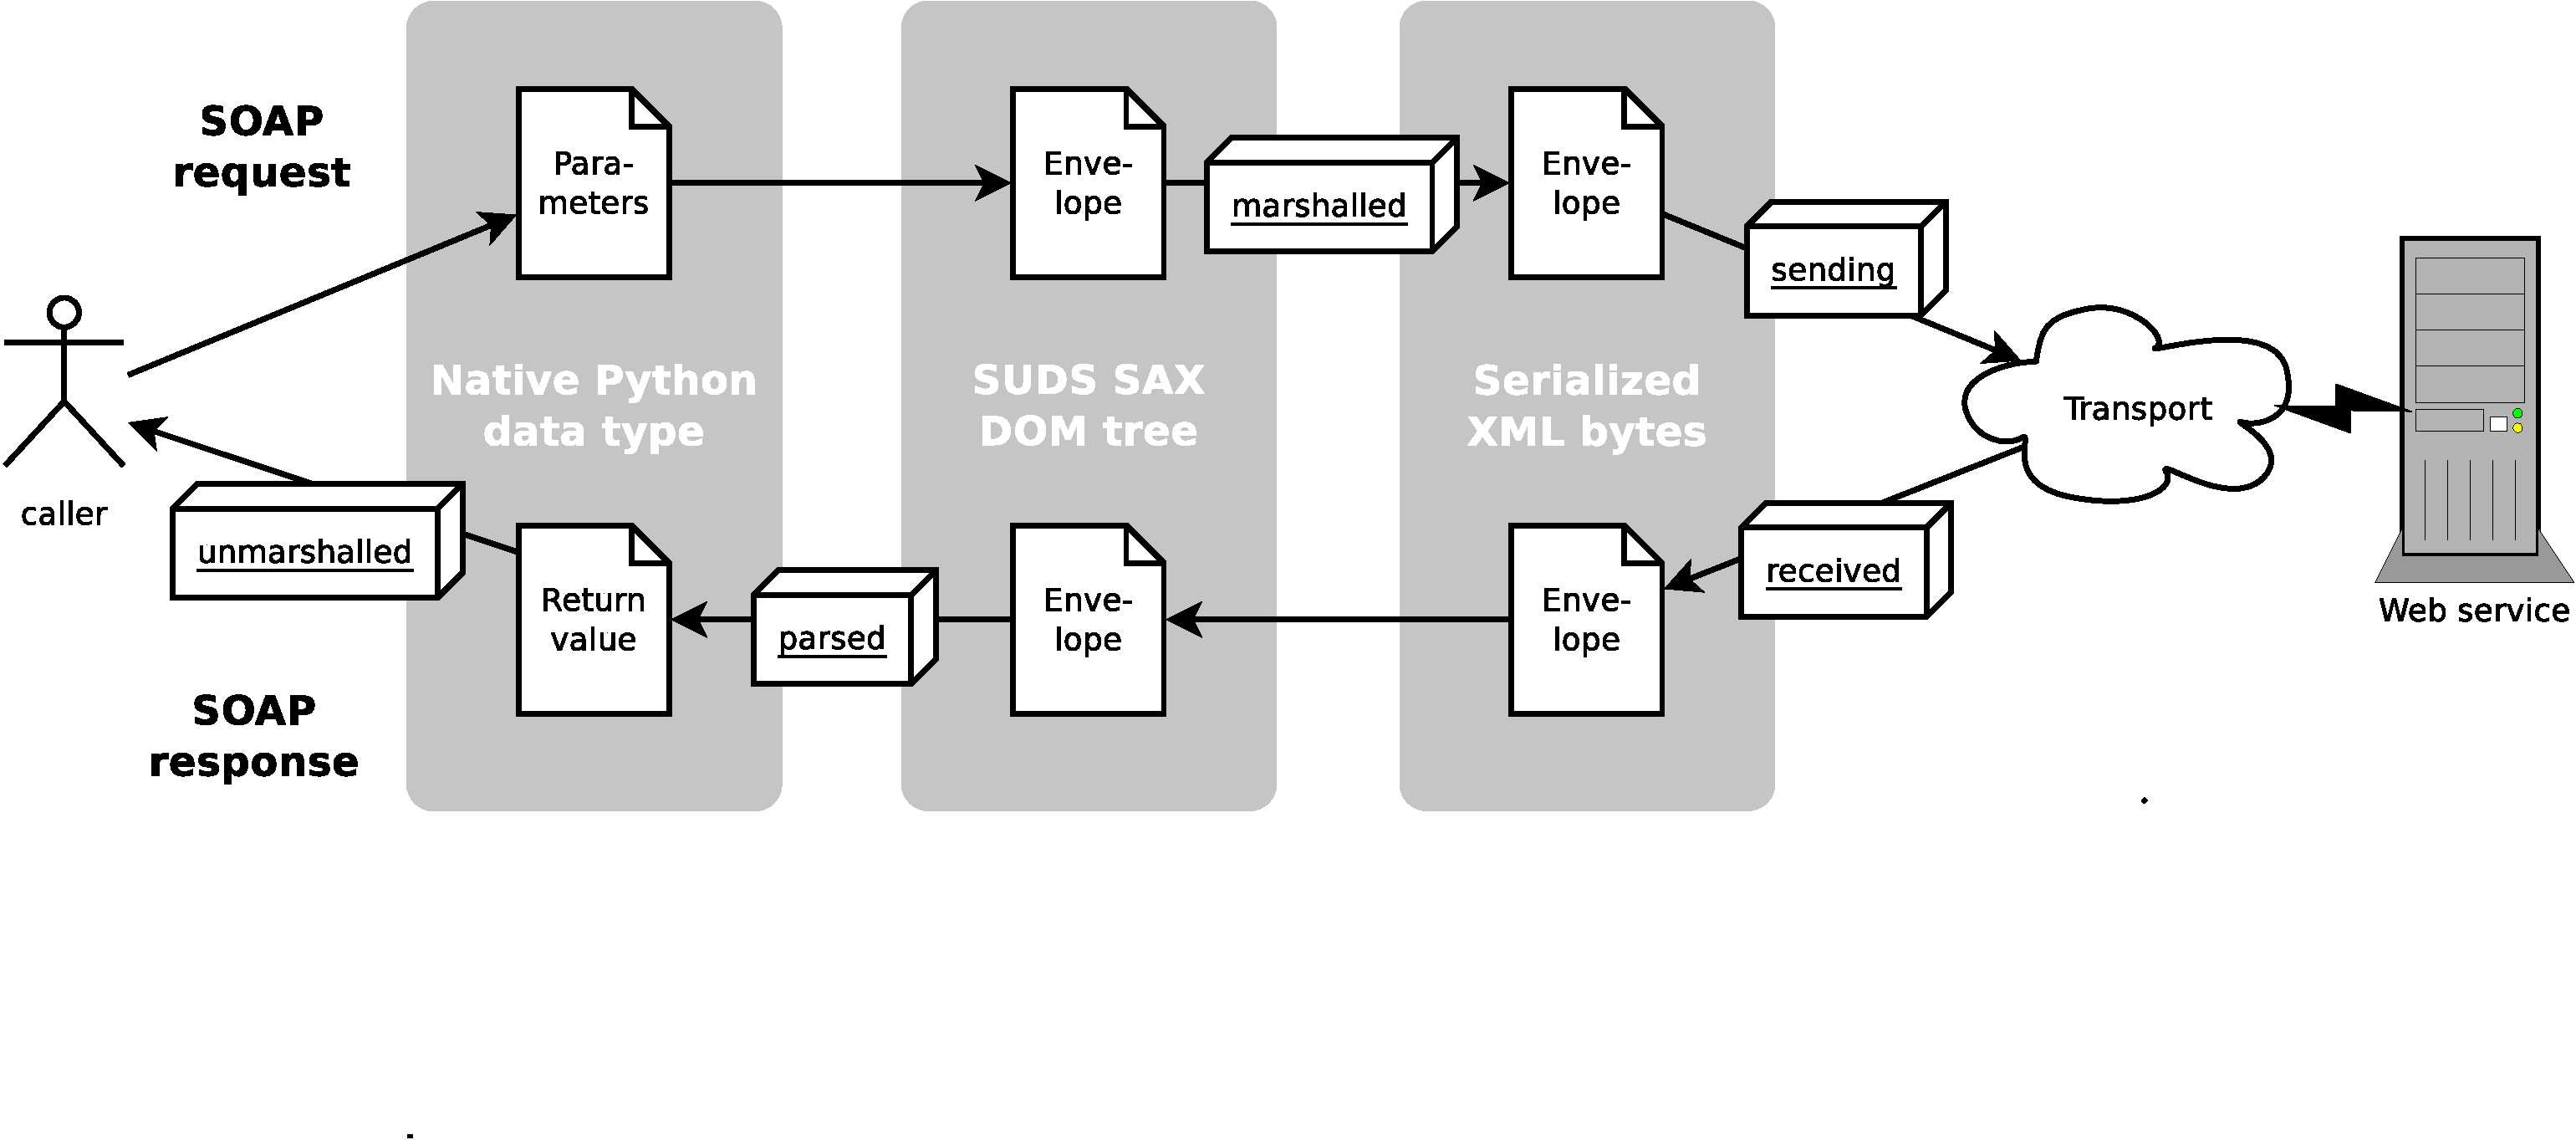
\includegraphics[width=\textwidth]{images/sudsMessage.pdf}
 \caption{SUDS message processing}
 \label{fig:sudsMessage}
\end{figure}
       %harmadik fejezet: eddig alkalmazott megoldas

\chapter{Improving SUDS}

\section{Implementing digital signatures -- SudsSigner}

\subsection{Internal structure}

The internal structure of the plugin can be seen on Figure \ref{fig:cmpdSudsSigner}, the stereotypes describe the functionality (component or binding) and the runtime environment (Python or native) of each component. Native components are preferred for their reusability and performance -- reusable components are tested more thoroughly, as more projects can depend on them, which makes them less prone to errors, thus more suitable for security-critical tasks, such as cryptography (OpenSSL). From a performance point of view, XML parsing and processing is also a task, that is better done using native and mature code (libxml2) because of its complexity. Python, on the other hand, is more suitable for the purpose of connecting components together, and describe high-level business logic in a readable and portable way.

\begin{figure}[htbp]
 \centering
 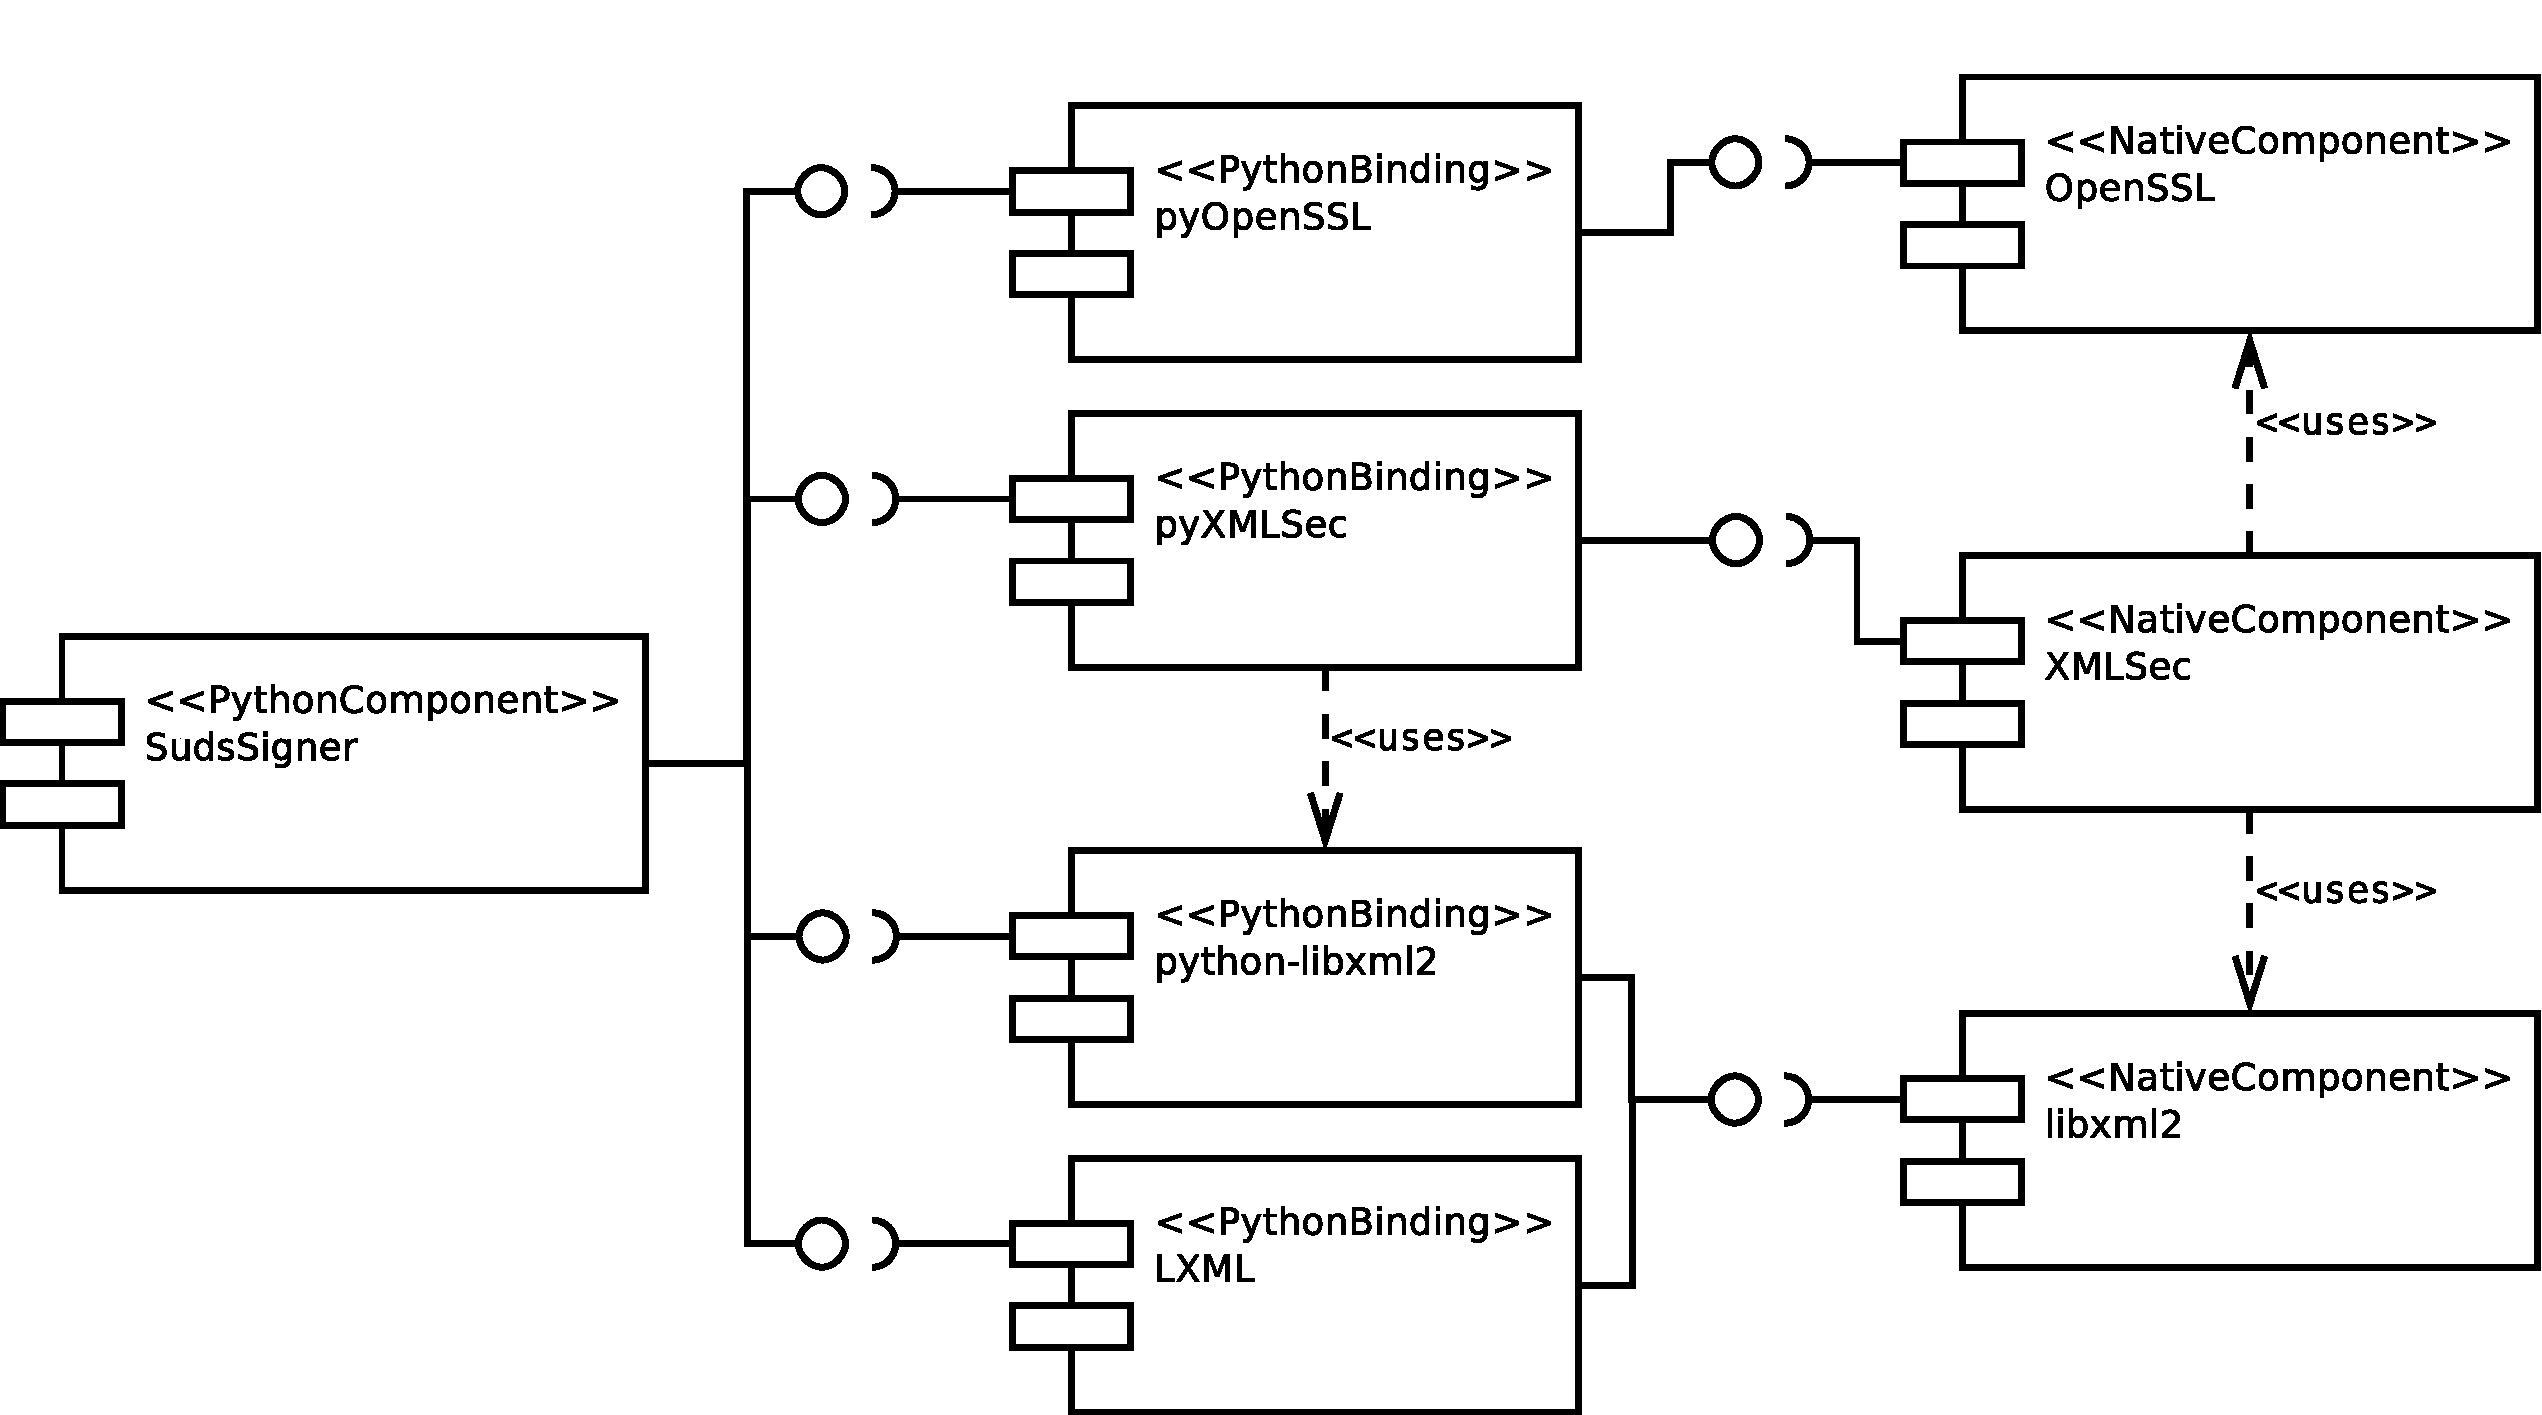
\includegraphics[width=\textwidth]{images/cmpdSudsSigner.pdf}
 \caption{Component diagram of the SudsSigner plugin}
 \label{fig:cmpdSudsSigner}
\end{figure}

\subsection{Components used}

\subsubsection{Libxml2, python-libxml2 and LXML}

``Libxml2 is the XML C parser and toolkit developed for the Gnome project (but usable outside of the Gnome platform), it is free software available under the MIT License.''\cite{libxml2-homepage} This sentence summarizes the project pretty well -- it's written in C, which is a good compromise between performance, portability and usability, and it's available under the MIT license, which makes it possible to either bundle it to FLOSS projects or redistribute it with proprietary software. Since many projects depend on it, the quality of the code is high, and it passes all of the OASIS XML Tests Suite.

Python-libxml2 provides low-level Python bindings to access all of the functionality of libxml2. It has the advantages that the developer gets the full power of libxml2, but the interface resembles the original C API, which causes longer development and debug cycles. On the other hand, LXML\cite{lxml-homepage} wraps libxml2 in modules and classes providing a powerful high-level interface, which is more suitable for quick prototyping and maintainable codebase -- one good example of this difference is python-libxml2 returning error codes versus LXML throwing exceptions in erroneus situations.

I chose this combination because no other combination can offer the perfomance of the native parsing and processing engine combined with so rich and powerful Python interface.

\subsubsection{OpenSSL and pyOpenSSL}

``The OpenSSL Project is a collaborative effort to develop a robust, commercial-grade, full-featured, and Open Source toolkit implementing [\ldots] a full-strength general purpose cryptography library''\cite{openssl-homepage} This library is also written in C, has a unique Apache and BSD-like license, and is FIPS 140-2 compliant. PyOpenSSL provides a friendly object-oriented interface, which makes it possible to access all the functionality of OpenSSL I needed. It's also well-maintained, which makes installing it on modern OSes a breeze. I chose this duo, because it seemed the only solution capable of handling PEM files in all the ways I needed.

\subsubsection{XMLSec and PyXMLSec}

XMLSec is a C library based on Libxml2 and supports XML signature, encryption, and canonicalization.\cite{xmlsec-homepage} It's released under the MIT license, and is still maintained, so most Linux distributions provide it as an easily installable package. It uses libxml2 for XML processing and it can use several cryptography backends (OpenSSL, GnuTLS, Libgcrypt, NSS) for signature creation and encryption.

Python bindings were created for the Glasnost project financed by the French Department of Economy, Finance and Industry in 2003, but development seems to ceased around 2005. The bindings are still working, only one feature needed a patch sent to the mailing list of the project in 2010. The documentation consists of a dozen examples and an API reference generated from the source code, so the use of these bindings require quite a bit of experimentation.

There are few other projects trying to create XML signatures, with not much success, so I chose this one, because at least it worked, and with a bit of work, I managed to make it do what I wanted.

\subsection{The Python component}

\begin{figure}[htbp]
 \centering
 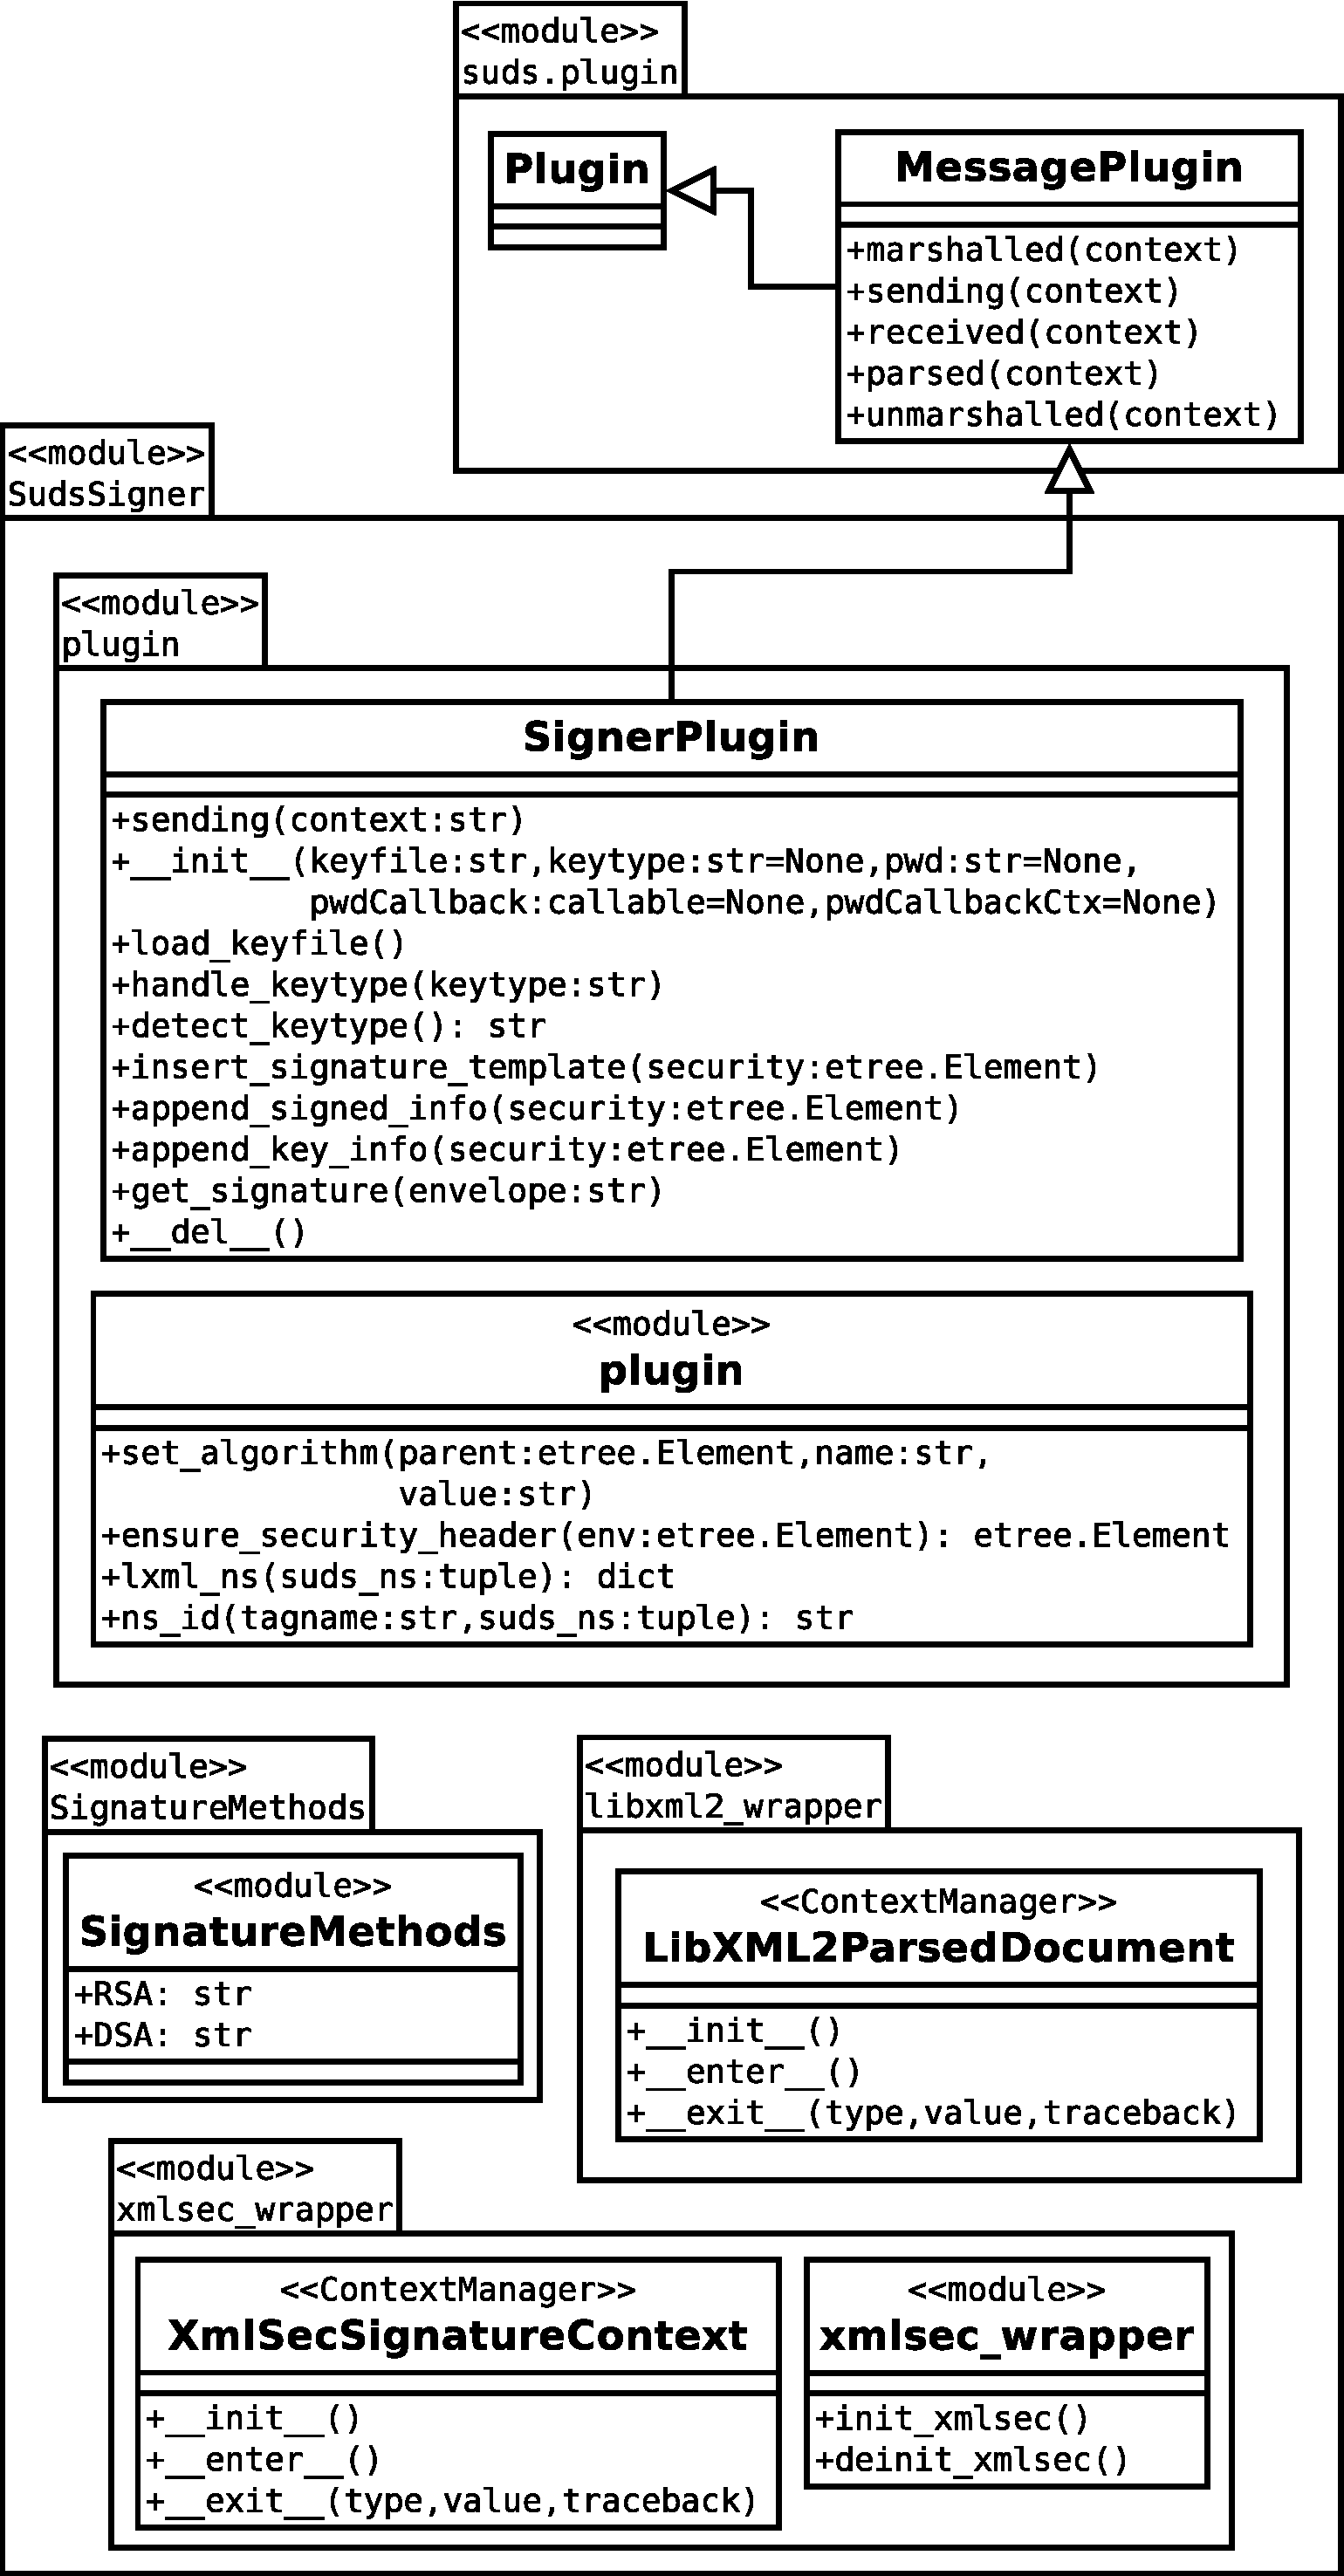
\includegraphics[height=22cm]{images/clsdSudsSigner.pdf}
 \caption{Class diagram of the SudsSigner Python component}
 \label{fig:clsdSudsSigner}
\end{figure}

The class diagram of the Python component of the plugin can be seen on Figure \ref{fig:clsdSudsSigner}, the Python-specific notations are expressed using stereotypes. Since UML doesn't support functions, just methods, each module with functions have a pseudoclass named after the module with \emph{module} stereotype. The main class is the \emph{SignerPlugin}, which directly interfaces SUDS, its \emph{sending} method is invoked after the SOAP envelope is complete, but before it's sent. The only parameter (\emph{context}) represents the SOAP invocation context, which makes the serialized envelope available through its \emph{envelope} attribute for access and modification. The method body is merely six lines of code, all elementary functionality is refactored to methods following the Single Reponsibility Principle (SRP), and the functionality can be described as two distinct steps.

\begin{enumerate}
 \item The first step does two things -- first, it finds and marks the body of the SOAP envelope with an ID (currently constant \verb|suds-signed|), then the security header is selected (or created if there's not one) and a so-called \emph{signature template} is inserted into it. This kind of processing is most easily done using the ElementTree implementation of LXML, therefore this part is framed with LXML parsing and serialization -- both the input and the output is an XML string.
 \item The second part finishes up, and signs the XML output using the template provided with the XMLSec library. The input and output are XML strings again, this time parsed directly by the libxml2 parser.
\end{enumerate}

Although the performance of the Python component is affected by its interpreted runtime, I made several architectural decisions to rationalize CPU and memory consumption. The \emph{SudsSigner} class initializes the native libraries only once in the constructor, and shuts them down in the destructor, thus reducing the time needed to process one single invocation. Native components need direct resource management because of the lack of garbage collection -- Python provides context managers for this problem, so I created two wrapper classes. \emph{LibXML2ParsedDocument} parses an XML string using python-libxml2, while \emph{XmlSecSignatureContext} encapsulates an XMLSec signature context object, and both free the resources upon leaving the scope of their use, thus minimizing memory usage.
       %negyedik fejezet: a jelolt megoldasa
%\chapter{Results}

\section{Timing measurement}

\subsection{Methodology}

I extended the \emph{Arena} testbed (see section \ref{arena}) with the option of measurement, which had a number of advantages. It ensured, that all runs were correct, and it already had the knowledge to arrange a ``rendezvous'' between services and consumers. The items added to the structure seen on Figure \ref{fig:clsdArena} were configurations and repeat values.

\begin{description}
 \item[Configurations] These define environment values, which are available to both the service and the consumer, thus are perfect to let them know about the parameters of the service. I defined the following suites to provide a way to get useful measurements.
 \begin{description}
  \item[No security] is without any form of authentication
  \item[Plain UsernameToken] uses UsernameToken with a plaintext password
  \item[Digest UsernameToken] uses UsernameToken with a digested password
  \item[Signed message] uses digital signature without a timestamp
  \item[Signed message w/ TS] uses digital signature with a timestamp
 \end{description}
 \item[Repeat values] The repeat values are important for the measurements to get a clear picture about the fixed and variable costs of the SOAP processing. I chose \textbf{1, 10 and 100}, as they provide reasonably fine enough resolution, while keeping runtime low.
\end{description}

\noindent
I put code into both consumers (CXF and SUDS) that measured two values.
\begin{description}
 \item[Proxy initialization] measures the time needed to create a proxy instance that can be used to invoke service methods. The measurement is started as the first statement after the entry point, and is stopped right after an instance of the service proxy is available in a local variable.
 \item[Invocation round-trip time] measures the time needed to invoke a service method one or more times. The measurement is started as the one for proxy initialization stops, and stops right after the last call has ended.
\end{description}

\noindent
In measurement mode, the \emph{Arena} testbed creates two files -- named using the timestamp at program startup -- a log file and a CSV table. The log file is written only by the \emph{Arena} measurement module, and currently contains one timestamped line for every test started. The CSV table on the other hand receives only the header from \emph{Arena}, its contents are produced by the consumers. They get the name of the CSV file and a prefix that contains the parameters of the current test through environment values, and using this, the two time measurements can be appended to the table. After the tests have run, the CSV table contains all the necessary data for timing analysis readable by any spreadsheet software.

\subsection{Environment}

For the sake of simplicity, I kept the setup used by \emph{Arena}, so the service and the consumer under test ran on the same host, and the loopback interface was used for network interconnection. The full network traffic of the measurement was captured using Wireshark and saved for later analysis -- this way, its overhead affected all test runs equally. This made it also easy to check later, that no other traffic went through the loopback interface used, thus providing equal circumstances. The exact components along with their version numbers and relations can be seen on Figure \ref{fig:measurenv} and Table \ref{tab:measurenv}. Note, that the composite relationship between the \emph{Arena} and the other processes describes the one between a process and a subprocess, while the cloud and the lightning symbols represent the network interconnectivity through the loopback interface, which is ``bootstrapped'' using information passed through environment values.

\begin{figure}[htbp]
 \centering
 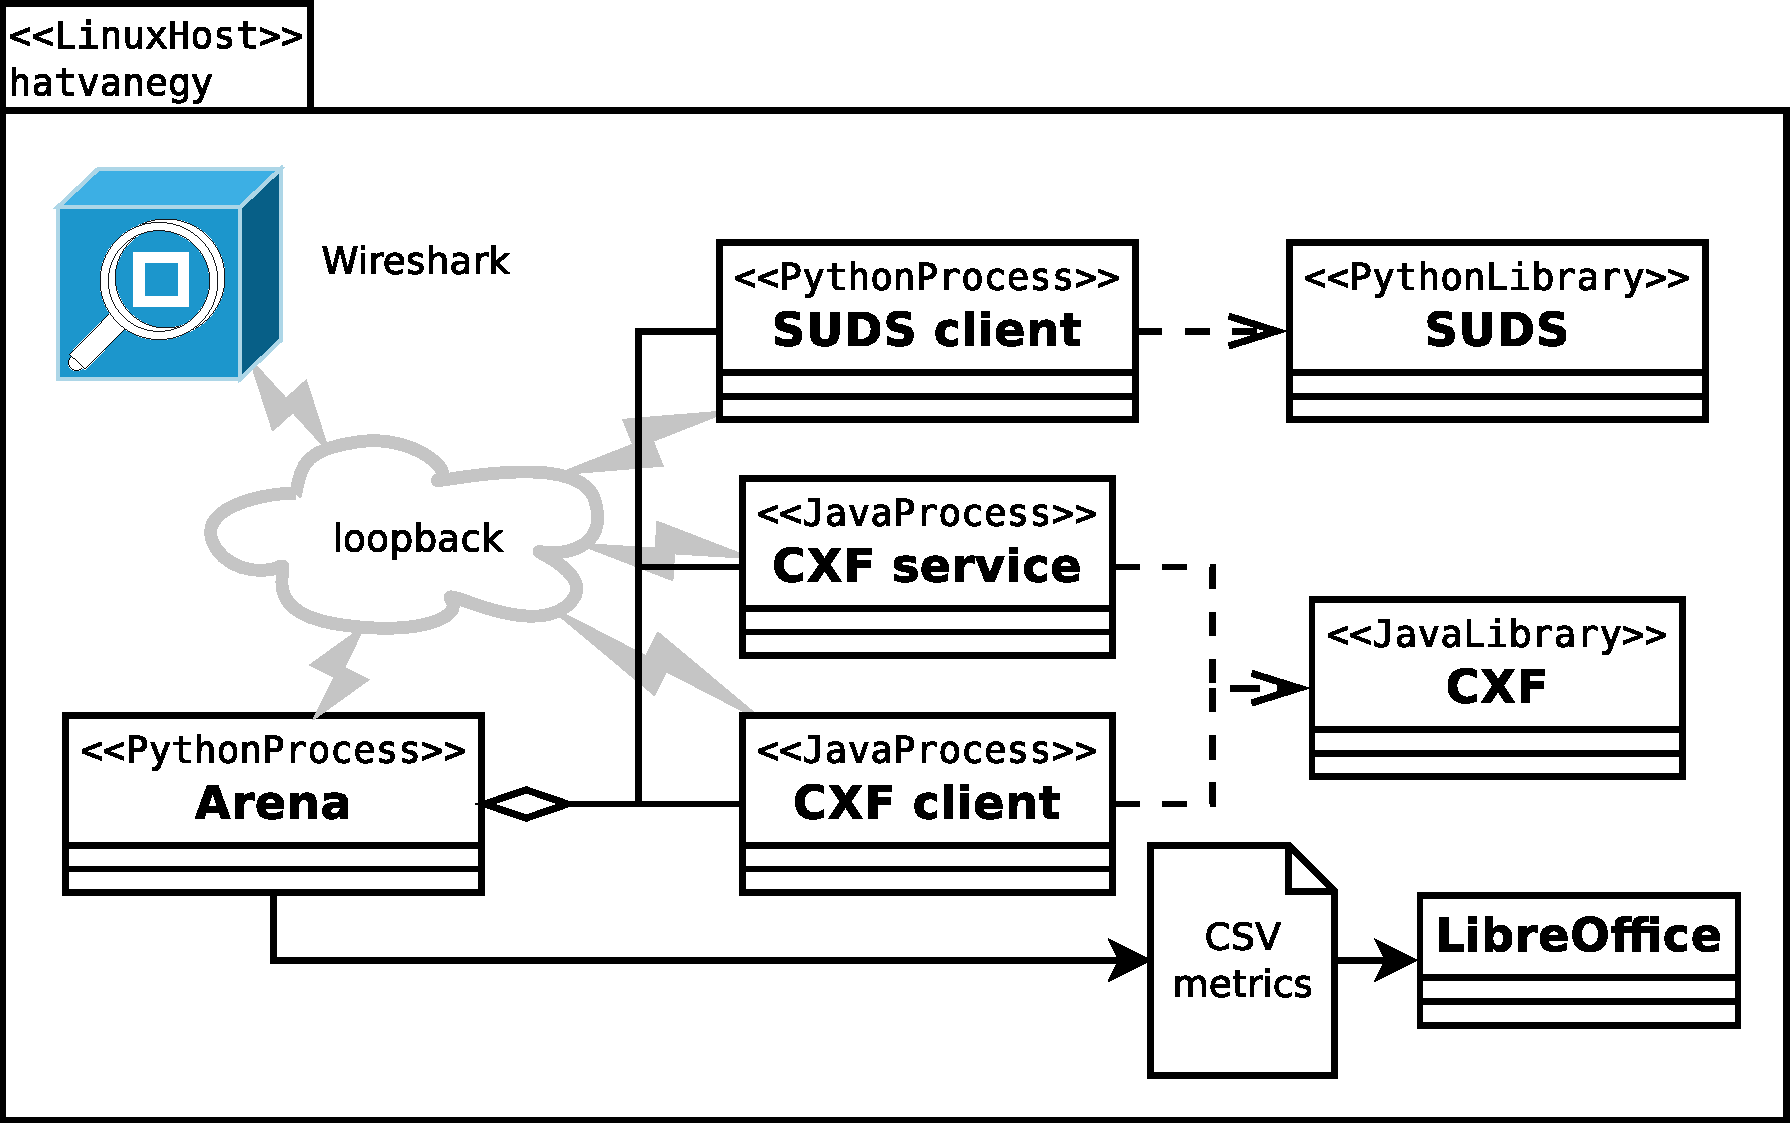
\includegraphics[width=0.9\textwidth]{images/measurenv.pdf}
 \caption{Structural diagram of the measurement environment}
 \label{fig:measurenv}
\end{figure}

\begin{table}[htbp]
 \centering
 \toprule
 \begin{minipage}[t]{0.55\linewidth}
  \centering
  \begin{tabular}{rl}
  \textbf{CPU} & Intel Core 2 Duo T7300 @ 2 GHz \\
  \textbf{RAM} & 4 GB \\
  \textbf{OS} & Debian GNU/Linux 7.0 ``Wheezy'' \\
  \textbf{Kernel} & Linux 3.1.0 / i686 \\
  \textbf{JRE} & Oracle Java SE 1.6.0\_26 \\
  \end{tabular}
 \end{minipage}
 \begin{minipage}[t]{0.3\linewidth}
  \centering
  \begin{tabular}{rl}
  \textbf{CXF} & 2.5.0 \\
  \textbf{Python} & 2.7.2 \\
  \textbf{SUDS} & 0.4.1 \\
  \textbf{Wireshark} & 1.7.0 \\
  \textbf{LibreOffice} & 3.4.4
  \end{tabular}
 \end{minipage}
 \bottomrule
 \caption{Attributes and version numbers of the measurement environment}
 \label{tab:measurenv}
\end{table}

\section{Timing analysis}

\subsection{Network traffic}
\label{traffic}

\begin{table}[htbp]
 \begin{center}
  \input{stat_packet}
  \caption{Network traffic generated by CXF and SUDS invocation}
  \label{tab:stat_packet}
 \end{center}
\end{table}

\noindent
The amount of network traffic generated by an invocation becomes less of an issue as network throughtput and latency continuously gets improved, although having perfect interconnections in every part of the system is far from reality. I used the TCP conversations module of the Wireshark analysis module, and put the results into Table \ref{tab:stat_packet}, which highlights a serious issue. Even in case of a single request, SUDS generates 33\% more packets as CXF, and at 100 requests, the difference becomes 250\%. The cause is simple; the current implementation of SUDS uses \emph{urllib2}, part of the Python base library, as I wrote in section \ref{sudsInvocation}. This solution opens a new TCP connection for each HTTP request by default, which causes overhead, especially a problem in case of HTTPS, which requires a TLS handshake in addition to the TCP one. Since this disadvantage of SUDS is unrelated to its architecture, I propose a soluton in Section \ref{keepalive}.

\subsection{Proxy initialization}

\begin{table}[htbp]
 \begin{center}
  \input{stat_init}
  \caption{Time needed for CXF and SUDS proxy initialization}
  \label{tab:stat_init}
 \end{center}
\end{table}

\noindent
The first thing that catches the eye on Table \ref{tab:stat_init} is that SUDS instantiates the proxy in less then half the time CXF needs to perform the same, regardless the configuration. It's also interesting to see, that according to these timings, SUDS needs an additional \mbox{210 ms} on average in case of digital signatures, whereas CXF takes roughly the same time in every case. The most logical explanation to me is that in the SUDS client, library import is done on demand, so this extra time is what it takes to load the LXML, libxml2 and XMLSec libraries, latter two requiring native components.

\subsection{Invocation round-trip time}

\begin{table}[htbp]
 \begin{center}
  \input{stat_invoke}
  \caption{Time needed for CXF and SUDS invocation}
  \label{tab:stat_invoke}
 \end{center}
\end{table}

\noindent
Per-invocation round-trip times are more interesting to architects, especially when designing consumers with more than one call to the service, and Table \ref{tab:stat_invoke} shows interesting differences between the two solutions. In case of a single invocation, CXF takes double the time SUDS needs, but this gain decreases with the number of requests increasing, and at 100 calls without digital signatures, CXF performs 1--5\% better. On the other hand, even 100 digitally signed messages are handled in almost 10\% less time by SUDS, probably caused by the elevated use of native components.

\section{Architectural differences}

\subsection{Runtime}

% VM startup time & memory consumption

\subsection{Use of native components}

% performance vs crashing

\chapter{Summary}

\section{Results summary}

\section{Future development opportunities}

Since most of the solutions in the Python ecosystem are free software in both senses\footnote{free as in free beer vs. free as in free speech}, software is continuously improved by its community following the needs of their members. For instance, during my thesis, I also created and published a proof-of-concept code to handle messages with attacments, and an interested user developed it further since to the point of real world usability. The following three goals are those, I think can and should be done in order to further improve Python SOA solutions.

\subsection{Short-term: taking advantage of HTTP keep-alive}
\label{keepalive}

The HTTP implementation used by SUDS generates network overhead, as I shown in section \ref{traffic}. Several ways exist to solve this issue -- as explained in \cite{so-1037406} -- some require replacing \emph{urllib2} with a whole new library, others just require extending it with plugins (so-called \emph{openers}) -- two things are for sure; it requires more than a simple method call, and the solution must be carefully tested for compatibility with different versions of its dependencies. Still, it only affects a relatively isolated part of the codebase, and would improve performance regardless of any optional (security) features.

\subsection{Mid-term: implementing XML encryption}

As I mentioned in section \ref{xmlenc}, as of 2011, the XML encryption standard is considered broken, so implementing it would do little or no good -- in my opinion, false belief in security is worse than no security at all. But as the future goes, XMLSec supports XML encryption, so in case the library is updated against the new design, it'd be fairly straightforward to make use of it in SUDS and sec-wall. I consider it a mid-term goal, since in this case (in contrast with digital signature), it makes more sense to use encryption on the response too, so the solution should be usable in both scenarios. By looking at Figure \ref{fig:sudsMessage}, it's clear, that the \emph{received} hook could be used to construct a message plugin the same way I did implementing the \emph{SudsSigner}.

\subsection{Long-term: wider cryptographic backend support}

The current \emph{SudsSigner} implementation supports only DSA and RSA digital signatures, and while these are quite common because of the ubiquity of PKI implemented with X.509 certificates, the WS\hyp{}Security standard -- or more specifically, the XML Signature W3C Recommendation -- contains guidelines for OpenPGP, too. As the main developer, Aleksey Sanin wrote in \cite{aleksey-pgp-mail}, XMLSec could have had PGP support, but he had problems regardning the availability and licensing of the necessary library. Two years later, John Belmonte wrote in \cite{belmonte-pgp-mail}, that he took part in a project that implemented PGP XML digital signatures in Python, although it seems by his words, that the product is closed source. That said, it doesn't seem impossible to add PGP support into XMLSec, using an appropriate library -- and GPGME \cite{gpgme-homepage} seems like the best candidate.
       %Osszefoglalas: ertekeles, tovabbi munka

%\include{08_utozm}     %Utolso lapok: koszonetnyilvanitas, egyeb...


%Megjegyzés: célszerű használni BibTeX-et:

%(pl. egyszeru stilus:):
%\bibliography{mybib}
%\bibliographystyle{alpha}

%(pl. harvard stílus -- ez esetben a harvard.sty is betoltendo):
%\bibliography{mybib}
%\bibliographystyle{dcu}


\begin{thebibliography}{99}
\addcontentsline{toc}{chapter}{\bibname}

\bibitem{soa_modeling}
Bell, Michael (2008) -- Service-Oriented Modeling: Service Analysis, Design, and Architecture. Wiley & Sons. pp. 3. ISBN 0-470-14111-3.

\bibitem{devcom_soa_intro}
Stevens, Michael (April 16, 2002) -- Service-Oriented Architecture Introduction
\url{http://www.developer.com/services/article.php/1010451/Service-Oriented-Architecture-Introduction-Part-1.htm}

\bibitem{ibm_soa_impro}
Balzer, Yvonne (July 16, 2004) -- Improve your SOA project plans\\
\url{http://www.ibm.com/developerworks/webservices/library/ws-improvesoa/}

\bibitem{box_soap_history}
Box, Don (April 4, 2001) -- A Brief History of SOAP\\
\url{http://www.xml.com/pub/a/ws/2001/04/04/soap.html}

\bibitem{acm-xmlenc-breaking}
``Jager, Tibor and Juraj, Somorovsky -- How to break XML encryption'',
CCS '11 Proceedings of the 18th ACM conference on Computer and communications security,
ACM New York, \mbox{ISBN 1-450-30948-6}

\bibitem{python-faq}
General Python FAQ, Python Software Foundation\\
\url{http://docs.python.org/faq/general#what-is-python}

\bibitem{so-206154}
What's the best SOAP client library for Python, and where is the documentation for it?, Stack Overflow\\
\url{http://stackoverflow.com/questions/206154/#206964}

\bibitem{pywebsvcs-talk}
Web Services for Python Email Archive, SourceForge\\
\url{http://sourceforge.net/mailarchive/message.php?msg_id=28266815}

\bibitem{zsi-doc}
Salz, Rich -- ZSI: The Zolera Soap Infrastructure\\
\url{http://pywebsvcs.sourceforge.net/zsi.html}

\bibitem{zsi-velocity}
Comparing WSDL & SOAP libraries, Velocity Reviews\\
\url{http://www.velocityreviews.com/forums/t336483-comparing-wsdl-and-soap-libraries.html}

\bibitem{soaplib2-changelog}
Change Log, soaplib v2.0.0beta documentation\\
\url{http://soaplib.github.com/soaplib/2_0/pages/changelog.html}

\bibitem{suds-doc}
Documentation -- SUDS Trac\\
\url{https://fedorahosted.org/suds/wiki/Documentation}

\bibitem{sec-wall-homepage}
sec-wall :: Home\\
\url{http://sec-wall.gefira.pl/}

\bibitem{w3schools-domintro}
XML DOM Introduction, w3schools.com\\
\url{http://www.w3schools.com/dom/dom_intro.asp}

\bibitem{ibm-timestamp}
Adams, Holt (March 30, 2004) -- Best Practices for web services, Part 12: Web services security, Part 2, IBM developerWorks\\
\url{http://www.ibm.com/developerworks/webservices/library/ws-best12/}

\bibitem{msdn-wss}
Seely, Scott (October 2002) -- Understanding WS-Security, MSDN\\
\url{http://msdn.microsoft.com/en-us/library/ms977327.aspx}

\bibitem{libxml2-homepage}
The XML C parser and toolkit of Gnome\\
\url{http://www.xmlsoft.org/}

\bibitem{lxml-homepage}
lxml - Processing XML and HTML with Python\\
\url{http://lxml.de/}

\bibitem{openssl-homepage}
OpenSSL: The Open Source toolkit for SSL/TLS\\
\url{http://openssl.org/}

\bibitem{xmlsec-homepage}
XML Security Library\\
\url{http://www.aleksey.com/xmlsec/}

\bibitem{aleksey-pgp-mail}
Sanin, Aleksey (Jul 17, 2002) -- PGP support, XML Security Library Discussions\\
\url{http://www.aleksey.com/pipermail/xmlsec/2002/004344.html}

\bibitem{belmonte-pgp-mail}
Belmonte, John (May 29, 2004) -- PGP and XML Signature, XML Security Library Discussions\\
\url{http://www.aleksey.com/pipermail/xmlsec/2004/006278.html}

\bibitem{gpgme-homepage}
GnuPG Made Easy (GPGME)\\
\url{http://www.gnupg.org/related_software/gpgme/}

\end{thebibliography}
       %Irodalomjegyzek

%%Fuggelek

\appendix

\chapter*{Appendix}
 \addcontentsline{toc}{chapter}{Appendix}
 \markboth{\uppercase{Appendix}}{\uppercase{Appendix}}
%\chaptermark{Függelék}

\setcounter{chapter}{1}     %A betu lesz

\blankpage
      %Fuggelek cimlap
%\section{Availability of relevant source code}

\subsection{SUDS}

Although I sent the patches enabling SUDS to digitally sign messages on May 21, 2011, as of December 2011, there's been no response from the maintainers. Because of this, the only way to obtain this code is my git repository hosted on GitHub.

\bigskip

\begin{center}
 \begin{minipage}[c]{0.7\linewidth}
  \begin{tabular}{rl}
   \textbf{Web access:} & \url{https://github.com/dnet/suds} \\
   \textbf{Git URL:} & \url{git://github.com/dnet/suds.git} \\
   \textbf{License:} & GNU LGPL version 3 (as it's part of SUDS)
  \end{tabular}
 \end{minipage}
 \hspace{5mm}
 \begin{minipage}[c]{3cm}
  
\includegraphics[width=3cm]{images/qr/suds.png}
 \end{minipage}
\end{center}

\subsection{SudsSigner}

The component for creating WS\hyp{}Security digital signatures is implemented as a message plugin, and is to be considered a separate software. The source code can be downloaded from my git repository hosted on GitHub.

\bigskip

\begin{center}
 \begin{minipage}[c]{0.7\linewidth}
  \begin{tabular}{rl}
   \textbf{Web access:} & \small\url{https://github.com/dnet/SudsSigner} \\
   \textbf{Git URL:} & \small\url{git://github.com/dnet/SudsSigner.git} \\
   \textbf{License:} & MIT
  \end{tabular}
 \end{minipage}
 \hspace{5mm}
 \begin{minipage}[c]{3cm}
  
\includegraphics[width=3cm]{images/qr/sudsign.png}
 \end{minipage}
\end{center}

\subsection{PyXMLSec}

The Python bindings for XMLSec were unmaintained since 2005, and the functionality SudsSigner needs can be only achieved in recent Python environments using a patch posted on the mailing list. I imported the Subversion repository of the project, applied the patch from the mailing list, and published this version of the code in my git repository hosted on GitHub.

\bigskip

\begin{center}
 \begin{minipage}[c]{0.7\linewidth}
  \begin{tabular}{rl}
   \textbf{Web access:} & \small\url{https://github.com/dnet/pyxmlsec} \\
   \textbf{Git URL:} & \small\url{git://github.com/dnet/pyxmlsec.git} \\
   \textbf{License:} & GNU GPL version 2
  \end{tabular}
 \end{minipage}
 \hspace{5mm}
 \begin{minipage}[c]{3cm}
  
\includegraphics[width=3cm]{images/qr/pxsec.png}
 \end{minipage}
\end{center}
      %1. fuggelek
%\include{10_f2_me}      %2. fuggelek
%\include{10_f3_pr}      %3. fuggelek
%\include{10_f4_cd}      %4. fuggelek
%\include{10_f5_dk}      %5. fuggelek
%\include{10_f6_hl}      %6. fuggelek
%\include{10_f7_br}      %Biralat: későbbi kötéshez, opcionalis

%%abrak, tablazatok jegyzeke

\addcontentsline{toc}{chapter}{List of Figures}
\listoffigures

\addcontentsline{toc}{chapter}{List of Tables}
\listoftables
        %Esetleges abrak, tablazatok jegyzeke (lehet az elejen is, nem kotelezo)

\chapter*{Abbreviations}
 \addcontentsline{toc}{chapter}{Abbreviations}
 \markboth{\uppercase{Abbreviations}}{}

\begin{tabular}{p{20mm}p{120mm}}

  CORBA & Component Object Request Broker Architecture \\
  DCOM & Distributed Component Object Model \\
  HTTP & Hypertext Transfer Protocol \\
  JKS & Java Key Store \\
  PEM & Privacy Enhanced Mail \\
  PHP & PHP: Hypertext Preprocessor \\
  RPC & Remote Procedure Call \\
  SOA & Service-oriented Architecture \\
  SOAP & Simple Object Access Protocol \\
  SRP & Single Responsibility Principle \\
  TCP & Transport Control Protocol \\
  UDDI & Universal Description Discovery and Integration \\
  W3C & World Wide Web Consortium \\
  WSDL & Web Services Description Language \\
  XML & Extensible Markup Language \\

\end{tabular}
      %Roviditesek jegyzeke

\end{document}
